\begin{figure}[h]
  \centering
   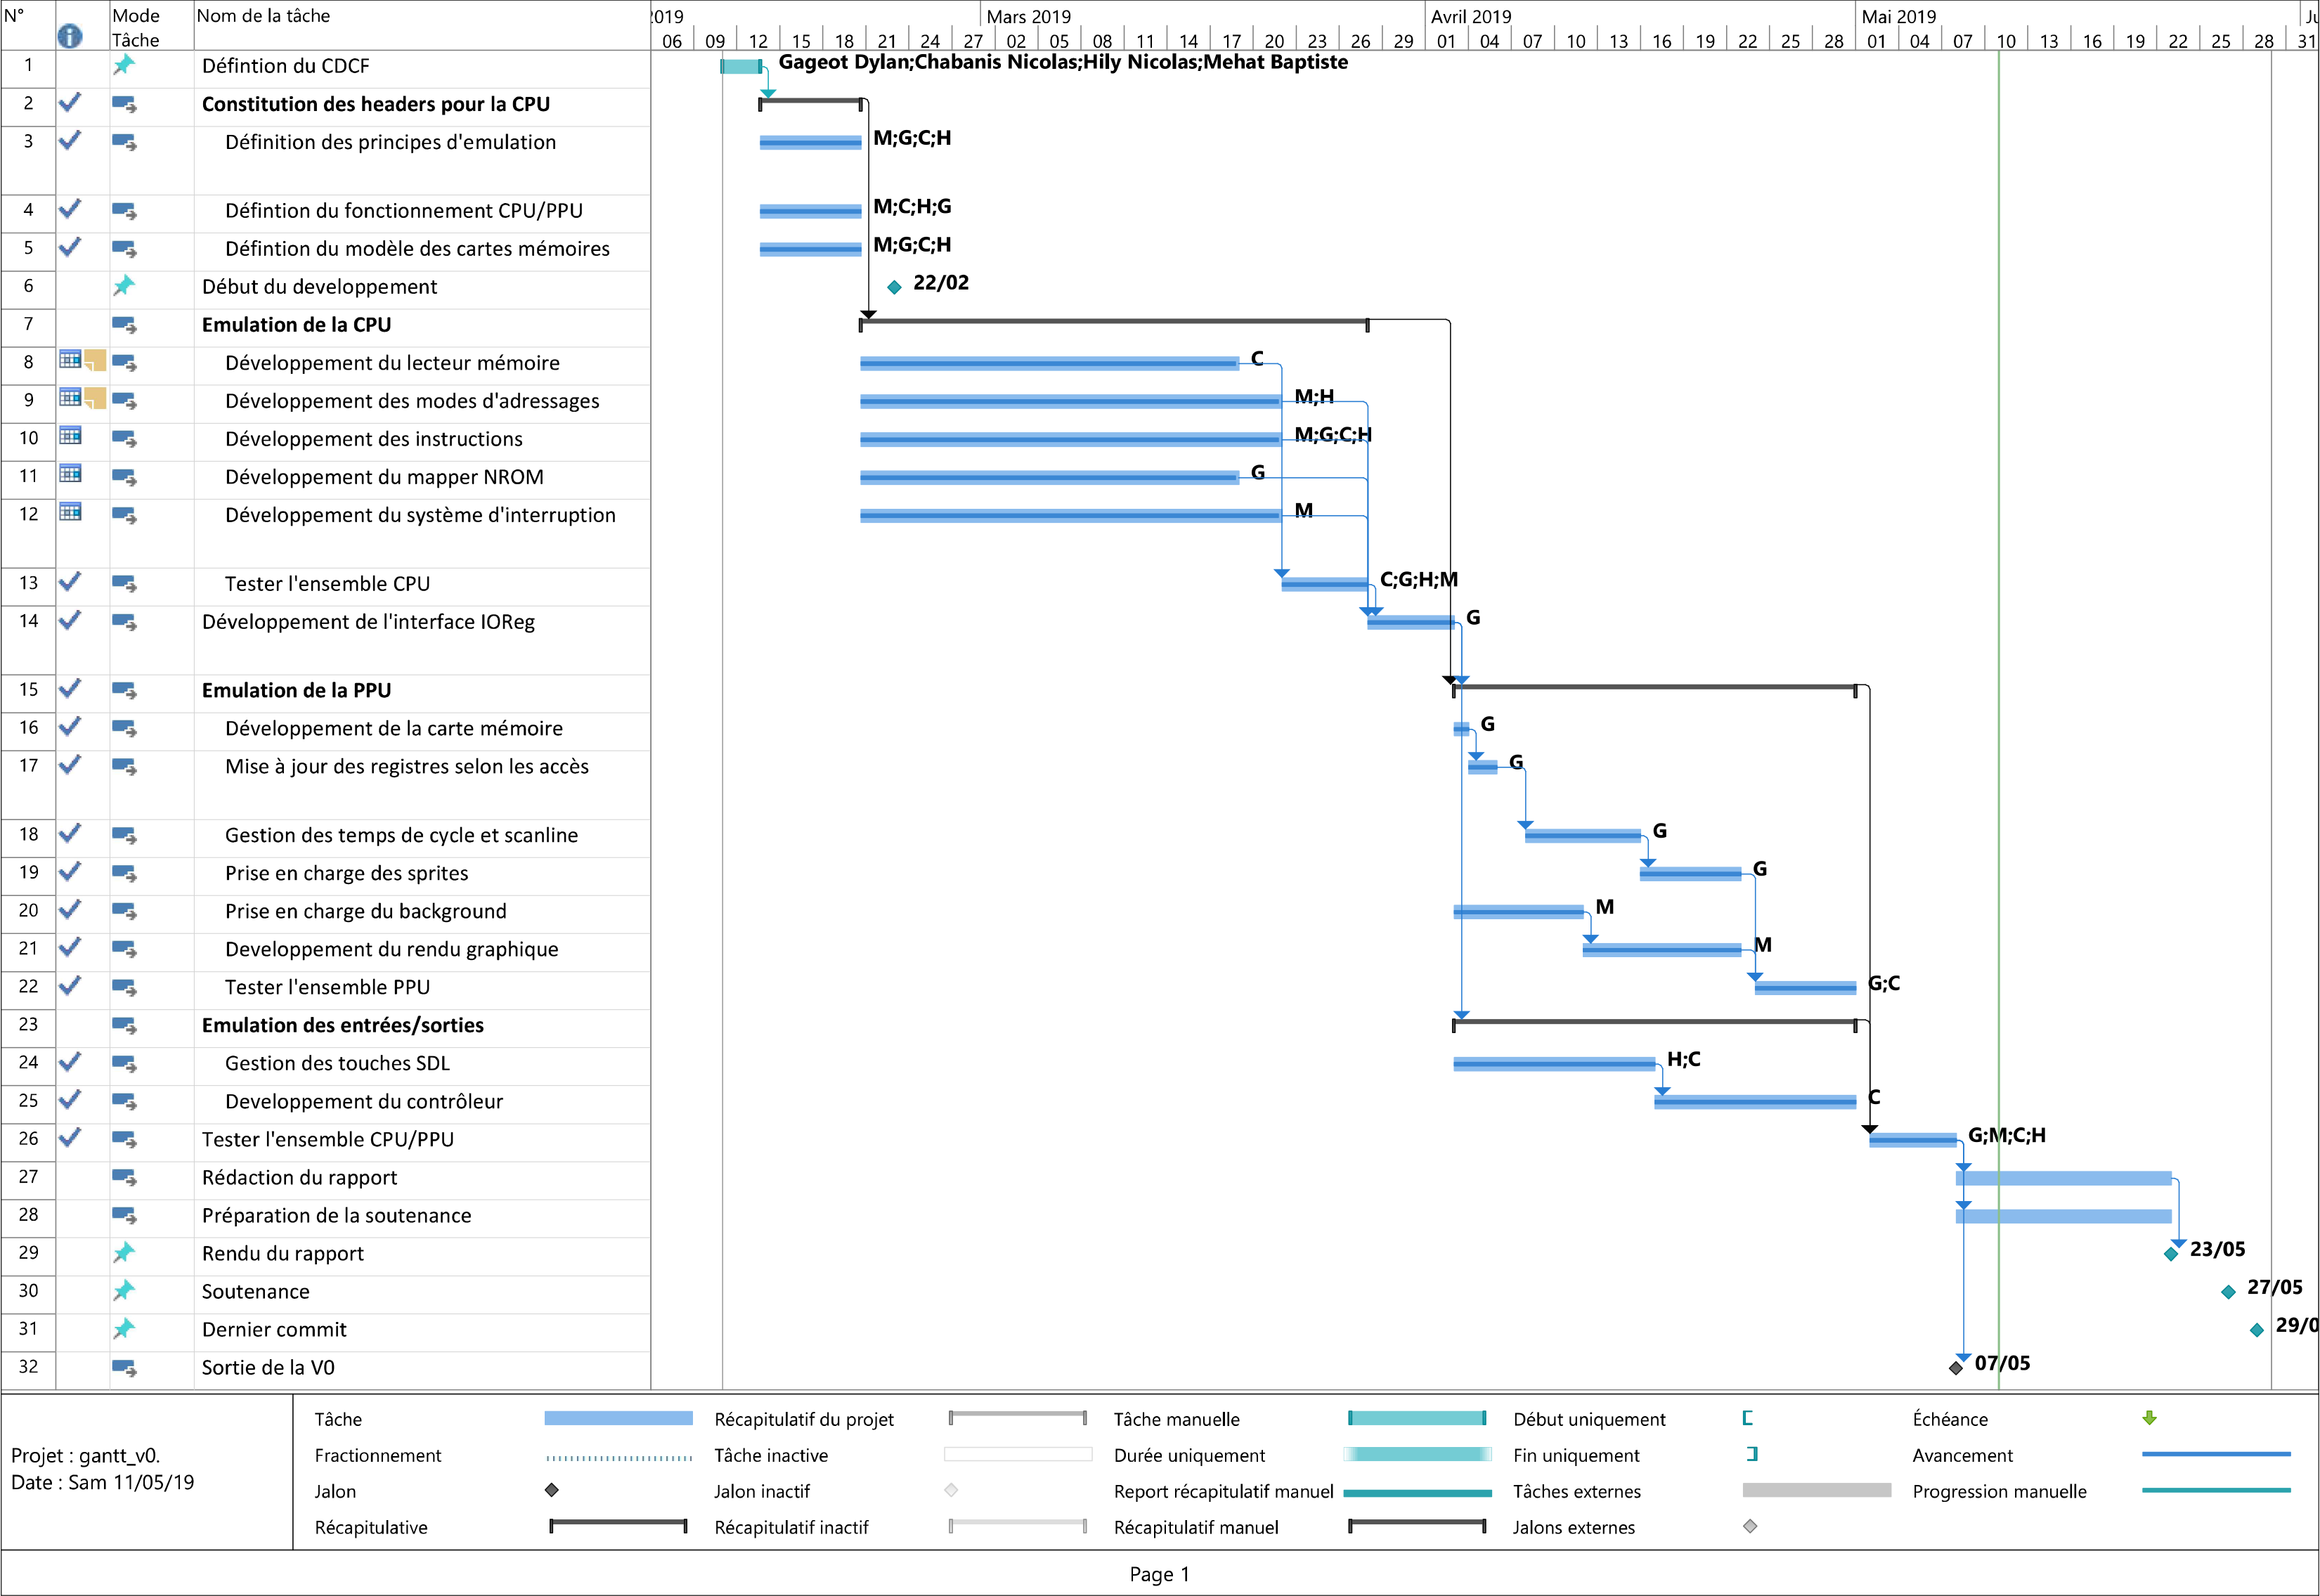
\includegraphics[scale=0.45]{GantV2.png}
   \caption{\label{étiquette} Diagramme de Gant de fin de Projet}
\end{figure}

Comme vous pouvez le voir en comparant le diagramme de gantt de début de projet et celui de fin de projet, celui-ci s'est déroulé en deux étapes contrairement aux trois prévues. Le développement de la CPU a été fait dans les échéances souhaitées. Cependant, par la suite, il a été décidé de revoir l'organisation sur le développement de la PPU et de l'IHM. En effet, lors de l'étude de la PPU, il est apparu plus simple que seulement deux personnes s'en occupent du fait de la complexité des liens existants entre chaque fonction codée. Ainsi, la PPU a été confiée à Dylan et Baptiste alors que Nicolas C et Nicolas H se sont concentrés sur la gestion des touches avec la SDL et le contrôleur. C'est donc le 7/05 que la V0 a été créée contrairement 29/04. La V1 contenant l'IHM a été totalement mise à l'écart de fait de la trop grande quantité de temps que cela demandait.
